\section{Possible CO Problems}
First, a review of several problems to understand how to \textbf{apply abstract ideas}; the objective is to \textbf{find and exploit relations} between known and new problems.\\
The same idea can have different effectiveness on different problems.\\

\subsection{Weighted set problems}
\subsubsection{The Knapsack Problem (KP)}
Finding how much "stuff" you can put in the sack.\\ 
Selecting from a set of object a \textbf{subset of maximum value} which can be \textbf{contained in a knapsack} of limited capacity. It consists of: 
\begin{itemize}
	\item a set $E$ of \textbf{elementary objects}
	\item a function $v: \, E \rightarrow \mathbb{N}$ describing the \textbf{volume of each object}
	\item a number $V \in \mathbb{N}$ describing the \textbf{capacity of the knapsack}
	\item a function $\phi : \, E \rightarrow \mathbb{N}$ describing the \textbf{value of each object}
\end{itemize}

The \textbf{ground set} is the set of \textbf{objects}, $B = E$.\\

The \textbf{feasible region} includes all \textbf{subsets of object} whose total \textbf{volume does not exceed the capacity of the knapsack}
$$ X = \left\{x \subseteq B : \, \sum_{j \in x} v_j \leq V \right\} $$

The \textbf{objective} is to \textbf{maximize the total value} of the chosen objects
$$ \max_{x \in X} f(x) = \sum_{j \in x} \phi_j $$

\newpage

\paragraph{Example} 	
\begin{center}
	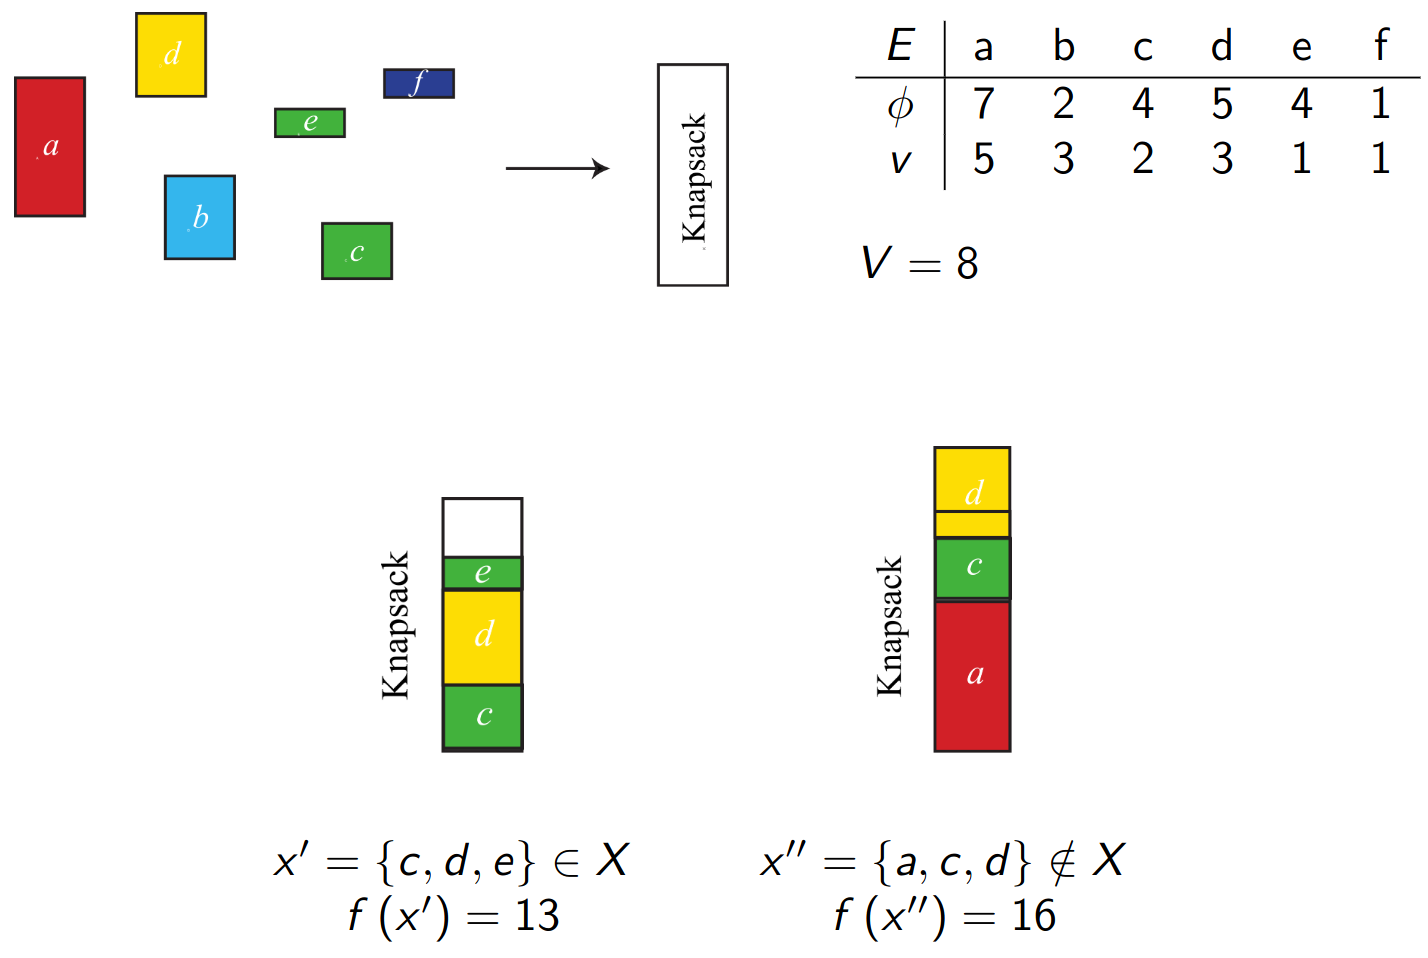
\includegraphics[width=\columnwidth]{img/KP1}
\end{center}
The left one is a solution, while the one on the right is not (or it can be called an unfeasible solution).

\newpage

\subsection{Set problems in metric spaces}
\subsubsection{Maximum Diversity Problem (MDP)}
Select the $k$ points with the maximum distance between each other.\\ 
Select \textbf{from a set of points} a \textbf{subset} of $k$ points with the\textbf{ maximum sum of all pairwise distances}. It consists of: 
\begin{itemize}
	\item a \textbf{set} $P$ of \textbf{points}
	\item a function $d: \, P \times P \rightarrow \mathbb{N}$ providing the \textbf{distance between point pairs}
	\item a number $k \in \left\{1, \, ... \, , |P| \right\}$ that is the \textbf{number of points} to select
\end{itemize}

The \textbf{ground set} is the set of \textbf{points} $B = P$.\\

The \textbf{feasible region} includes all \textbf{subset} of $k$ \textbf{points} 
$$ X = \left\{x \in B : \, |x| = k \right\}$$

The \textbf{objective} is to \textbf{maximize the sum} of all pairwise \textbf{distances} between the selected points
$$ \max_{x \in X} f(x) = \sum_{(i,j):i,j \in x} d_{ij}$$ 

\paragraph{Example}
\begin{center}
	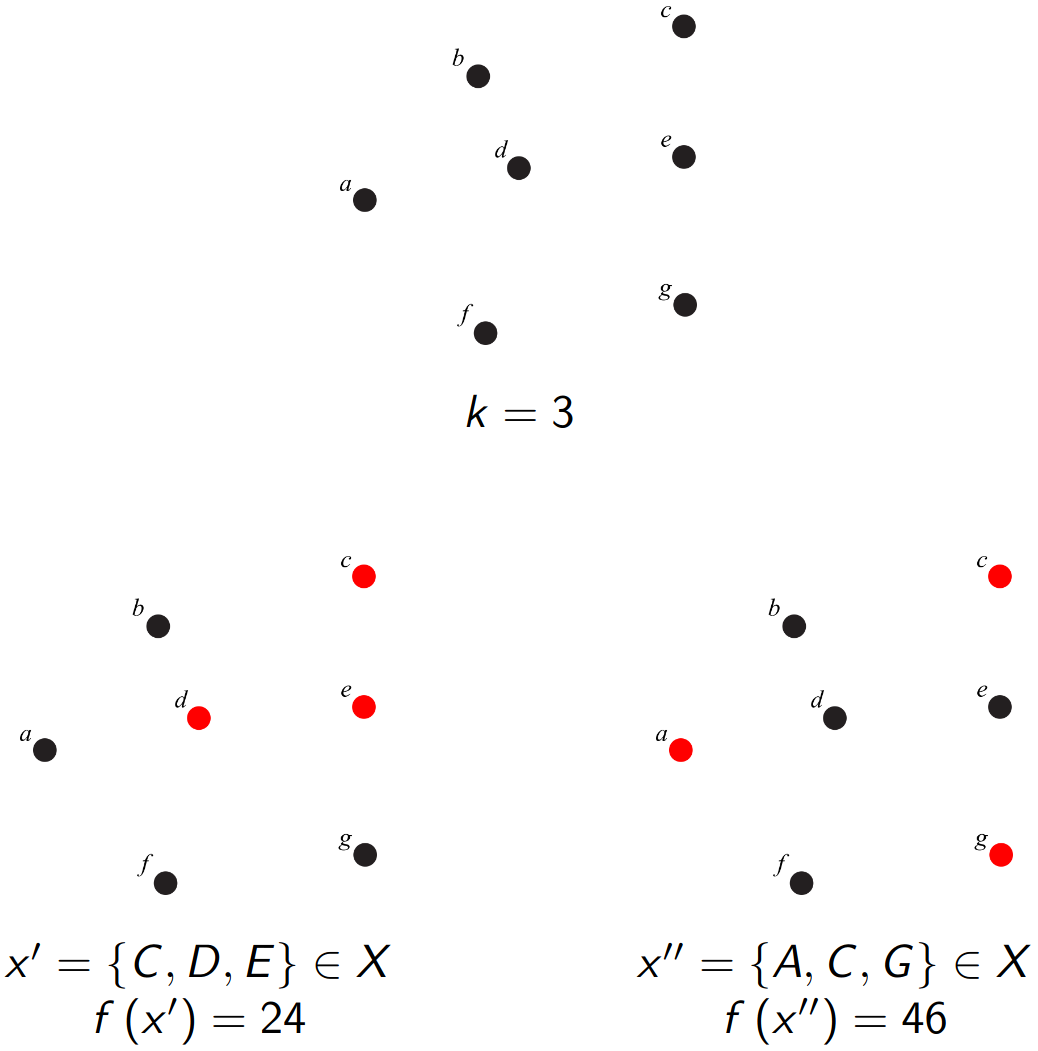
\includegraphics[width=0.6\columnwidth]{img/MDP1}
\end{center}

\newpage

\subsection*{Interlude 1: The objective function}
\addcontentsline{toc}{subsection}{Interlude 1: The objective function}
%\addcontentsline{toc}{subsection}{\protect\numberline{}Interlude: The objective function}
The \textbf{objective function} associates \textbf{integer values} to \textbf{feasible subjects}
$$ f: \, X \rightarrow \mathbb{N} $$
Computing the objective function can be complex (and exhausting).\\

In the cases seen before: 
\begin{itemize}
	\item the KP has an \textbf{additive} function which sums values of a function defined on the ground set (each element only has its own value)
	$$ \phi : \, B \rightarrow \mathbb{N} \; \text{ induces } \; f(x) = \sum_{j \in x} \phi_j : \, X \rightarrow \mathbb{N} $$
	the additive function is easy to recompute if the subset $x$ changes, just sum each element added and subtract each element removed.\\
	
	\item the MDP has a \textbf{quadratic} objective function (each point needs to have the distance to every other element). \\
	The process for recomputing, when the subset changes, is more complex, but still quadratic in nature.\\
\end{itemize}
Both of these functions are defined not only on $X$ but on the whole $2^B$ (is it useful?).\\

\newpage

\subsection{Partitioning set problems}
\subsubsection{Bin Packing Problem (BPP)}
Put a set of objects in the minimum possible number of containers of a given volume.\\ 
Divide a \textbf{set of voluminous objects} into the \textbf{minimum number of containers} of given capacity. It consists of:
\begin{itemize}
	\item a set $E$ of \textbf{elementary objects}
	\item a function $v: \, E \rightarrow \mathbb{N}$ describing the \textbf{volume of each object}
	\item a set $C$ of \textbf{containers}
	\item a number $V \in \mathbb{N}$ that is the \textbf{volume of the containers}
\end{itemize}

The \textbf{ground set} includes all \textbf{(object, container) pairs}, $B = E \times C$.\\

The \textbf{feasible region} includes all \textbf{partitions} of the \textbf{objects} among the \textbf{containers} not exceeding the capacity of any container
$$ X = \left\{ x \subseteq B : \, |x \cap B_e| = 1 \;\; \forall e \in E, \sum_{(e,c) \in B^c} v_e \leq V \;\; \forall c \in C \right\}$$
with $B_e \left\{(i,j) \in B : \, i = e\right\}$ and $B^c = \{(i,j) \in B : \, j = c \}$ (respectively, pairs in relation to the elements and pairs in relation to the containers).\\

The \textbf{objective} is to \textbf{minimize the number of containers} used
$$ \min_{x \in X} f(x) = \left| \left\{c \in C : \, x \cap B^c \neq \emptyset \right\}\right| $$
the cardinality of the set of containers $C$ such that the pairs of the solution intersect $B^c$ in at least one element (not empty).\\

\newpage

\paragraph{Example}
\begin{center}
	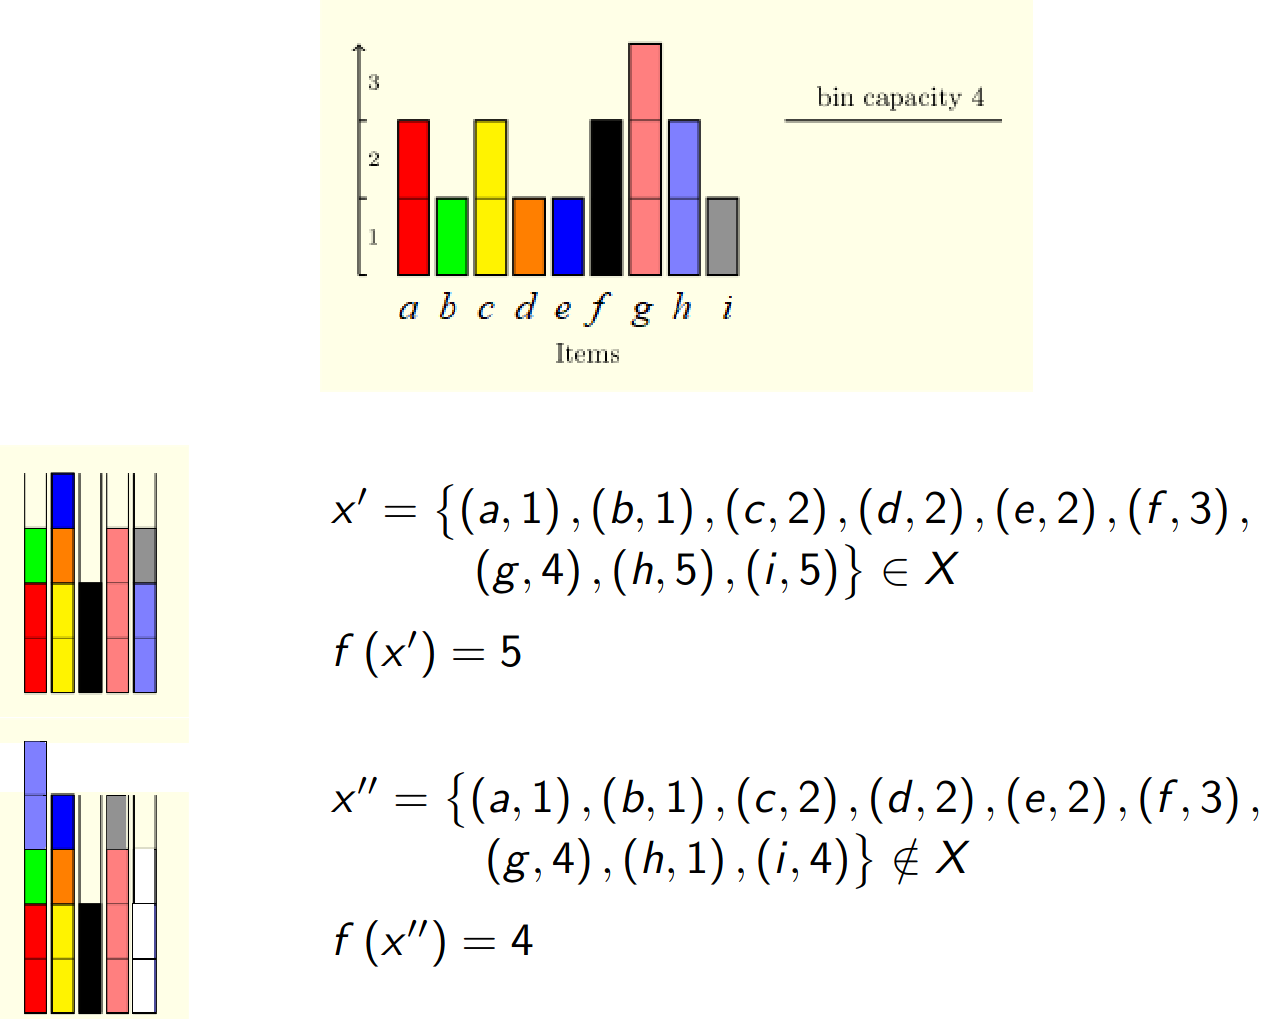
\includegraphics[width=\columnwidth]{img/BPP1}
\end{center}
In the first solution there is only a single pair for each item and the capacity of each container is not exceeded so it's a valid solution.

\newpage

\subsection{Parallel Machine Scheduling Problem (PMSP)}
Divide a \textbf{set of tasks} among a \textbf{set of machines} \textbf{minimizing the completion time}. It consists of: 
\begin{itemize}
	\item a set $T$ of \textbf{tasks}
	\item a function $d : T \rightarrow \mathbb{N}$ describing the \textbf{time length of each task}
	\item a set $M$ of \textbf{machines}
\end{itemize}
divide the tasks among the machines with the minimum completion time, each task to one machine only.\\

The \textbf{ground set} includes all \textbf{(task,machine) pairs}, $B = T \times M$.\\

The \textbf{feasible region} includes all \textbf{partitions of tasks among machines} (the order of the tasks is irrelevant, sum is the same)
$$ X = \left\{x \subseteq B : \, |x \cap B_t| = 1 \;\; \forall t \in T \right\}$$

The \textbf{objective} is to \textbf{minimize the maximum sum of time lengths} for each machine
$$ \min_{x \in X} f(x) = \max_{m \in M} \sum_{t:(t,m) \in x} d_t $$
this wants to minimize the maximum sum of duration for each machine in the solution; the final "value" (time spent) needs to be at a minimum, and it is determined only by the longest-running machine.

\newpage

\paragraph{Example}
\begin{center}
	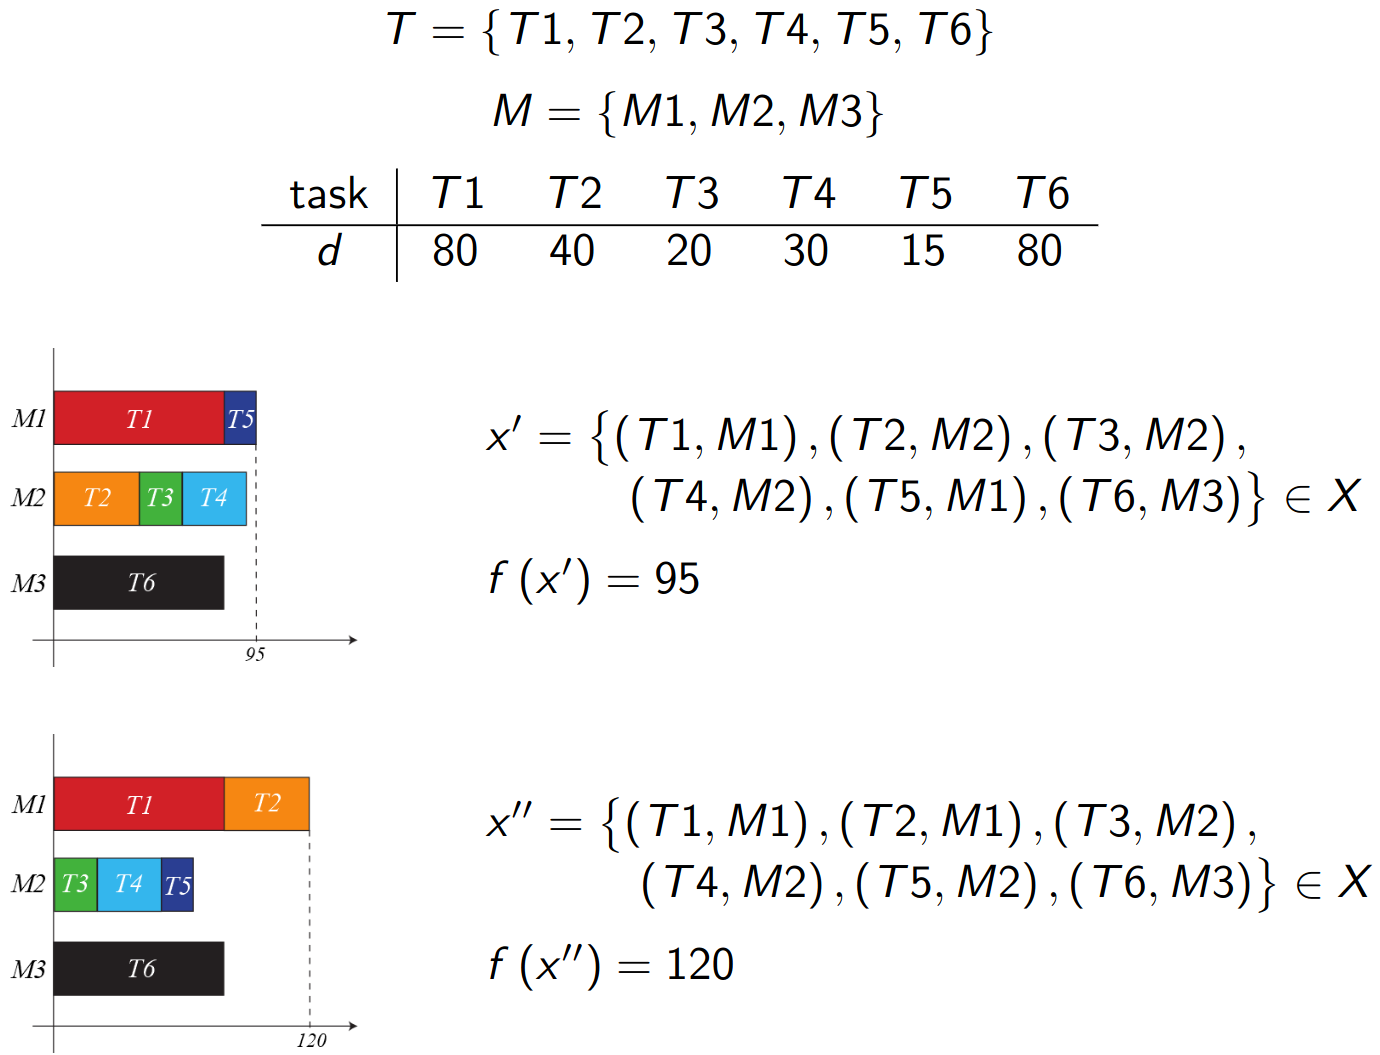
\includegraphics[width=\columnwidth]{img/PMSP}
\end{center}
The objective function wants to minimize the completion time, the value to complete the whole set of tasks, i.e. it wants to minimize the maximum time of a single machine.

\newpage

\subsection*{Interlude 2: The objective function again}
\addcontentsline{toc}{subsection}{Interlude 2: The objective function again}
The \textbf{ground set} is \textbf{not} always a single set, in the last examples was a Cartesian product of two sets. \\

The objective function for the BPP and PMSP is not additive and not trivial to compute. \\

Small \textbf{changes} in the solution have a \textbf{variable impact} on the objective, it can be: 
\begin{itemize}
	\item \textbf{equal} to the time length of the moved task (e.g., move $T5$ on $M1$ in $x''$)
	\item \textbf{zero} (e.g., move $T5$ on $M3$ in $x''$)
	\item \textbf{intermediate} (e.g., move $T2$ on $M2$ in $x''$)
\end{itemize}
The \textbf{impact} of a change to the solution \textbf{depends} both on the \textbf{modified} elements and the \textbf{unmodified} ones (contrary to the earlier interlude).\\

The objective function is "flat", there are \textbf{several solutions} with the same \textbf{value} (is there a way to tell if a change is "good"?).\\

\newpage

\subsection{Logic function problems}
\subsubsection{Max-SAT (satisfaction) problem}
Given a \textit{CNF} (Conjunctive Normal Form), assign truth values to its logical variables to satisfy the \textbf{maximum weight subset of its logical clauses}. It consists of: 
\begin{itemize}
	\item a set $V$ of \textbf{logical variables} $x_j$ with values in $\mathbb{B} = \{0, 1\}$ (\textit{false}, \textit{true}); the variables taken into consideration, which can be true or false
	\item a \textbf{literal} $l_j$ is a function consisting of an \textbf{affirmed or negated variable}
	$$ l_j (x) \in \{x_j, \overline{x}_j\}$$
	\item a \textbf{logical clause} is a disjunction or \textbf{logical sum} (\textit{OR}) \textbf{of literals}
	$$ C_i (x) = l_{i,1} \vee \; ... \; \vee l_{i,n}$$
	\item a \textbf{conjunctive normal form} (\textit{CNF}) is a conjunction or \textbf{logical product} (\textit{AND}) \textbf{of logical formulae}
	$$ CNF (x) = C_1 \wedge \; ... \; \wedge C_n $$
	it's the (logic) product of (logic) sums (literals).\\
	\item to satisfy a logical function means to make it assume value 1
	\item a function $w$ provides the \textbf{weights} of the \textit{CNF} formulae
\end{itemize}

The \textbf{ground set} is the set of \textbf{all simple truth assignments}
$$ B = V \times \mathbb{B} = \left\{(x_1, 0), (x_1, 1), \; ... \; , (x_n, 0), (x_n, 1)\right\}$$
the cartesian product of the set of variables with the set of logical values.\\

The \textbf{feasible region} includes all \textbf{subsets of simple assignments} that are:
\begin{itemize}
	\item \textbf{complete}, every variable has at least one value
	\item \textbf{consistent}, every variable has at most one value
\end{itemize}
$$ X = \left\{x \subseteq B : \, |x \cap B_v| = 1 \; \forall v \in V \right\}$$
with $B_{x_j} = \left\{(x_j, 0), (x_j, 1)\right\}$.\\

The \textbf{objective} is to \textbf{maximize the total weight of the satisfied formulae}: 
$$ \max_{x \in X} f(x) = \sum_{i:C_i(x) = 1} w_i $$
This is defined only on feasible solutions (you HAVE to assign a value to a variable, it just might not be the Max-SAT solution).\\

\paragraph{Example}
\begin{itemize}
	\item Variables
	$$ V = \{x_1, x_2, x_3, x_4\} $$
	\item Literals
	$$ L = {x_1, \overline{x}_1, x_2, \overline{x}_2, x_3, \overline{x}_3, x_4, \overline{x}_4} $$
	\item Logical clauses
	$$ C_1 = \overline{x}_1 \vee x_2 \;\;\;\; ... \;\;\;\; C_7 = x_2 $$ 
	\item Conjunctive normal form
	$$CNF = (\overline{x}_1 \vee x_2) \wedge (\overline{x}_1 \vee x_3) \wedge (\overline{x}_1 \vee \overline{x}_3) \wedge (\overline{x}_2 \vee x_4) \wedge (\overline{x}_2 \vee \overline{x}_4) \wedge x_1 \wedge x_2 $$
	\item Weight function (uniform, all 1):
	$$ w_i = 1 \;\;\;\;\;\; i = 1, \; ... \; ,7 $$
\end{itemize}
$x = \{(x_1, 0), (x_2, 0), (x_3, 1), (x_4, 1)\}$ satisfies $f (x) = 5$ formulae out of $7$.\\
Complementing a variable does not always change $f(x)$ ($x_1$ does, $x_4$ doesn't).\\

\newpage

\subsection{Numerical matrix problems}
\subsubsection{Set Covering (SCP)}
Given
\begin{itemize}
	\item a \textbf{binary matrix} $A \in \mathbb{B}^{m,n}$ with \textbf{row set} $R$ and \textbf{column set} $C$
	\item column $j \in C$ \textbf{covers} row $i \in R$ when $a_{ij} = 1$
	\item a function $c :\, C \rightarrow \mathbb{N}$ provides the \textbf{cost of each column}
\end{itemize}
Select a \textbf{subset of columns covering all rows at minimum cost}.\\

Essentially: there's a binary matrix (filled with 0s and 1s), each column has a cost, you need to get the minimum cost for covering all the rows, i.e. having at least one "1" value for each row.\\

The \textbf{ground set} is the set of \textbf{columns}, $B = C$.\\

The \textbf{feasible region} includes all \textbf{subsets} of \textbf{columns} that \textbf{cover all rows}
$$ X \left\{ x \subseteq B : \, \sum_{j \in x} a_{ij} \geq 1 \; \forall i \in R \right\}$$
All the solution subset of the columns such that there is at least a 1 ($a_{ij} \geq 1$) for all rows $i$.\\

The \textbf{objective} is to \textbf{minimize} the total \textbf{cost} of the selected \textbf{columns}
$$ \min_{x \in X} f(x) = \sum_{j \in x} c_j$$
It's additive and is simply the cost of the columns.\\

\newpage

\paragraph{Example}
\begin{center}
	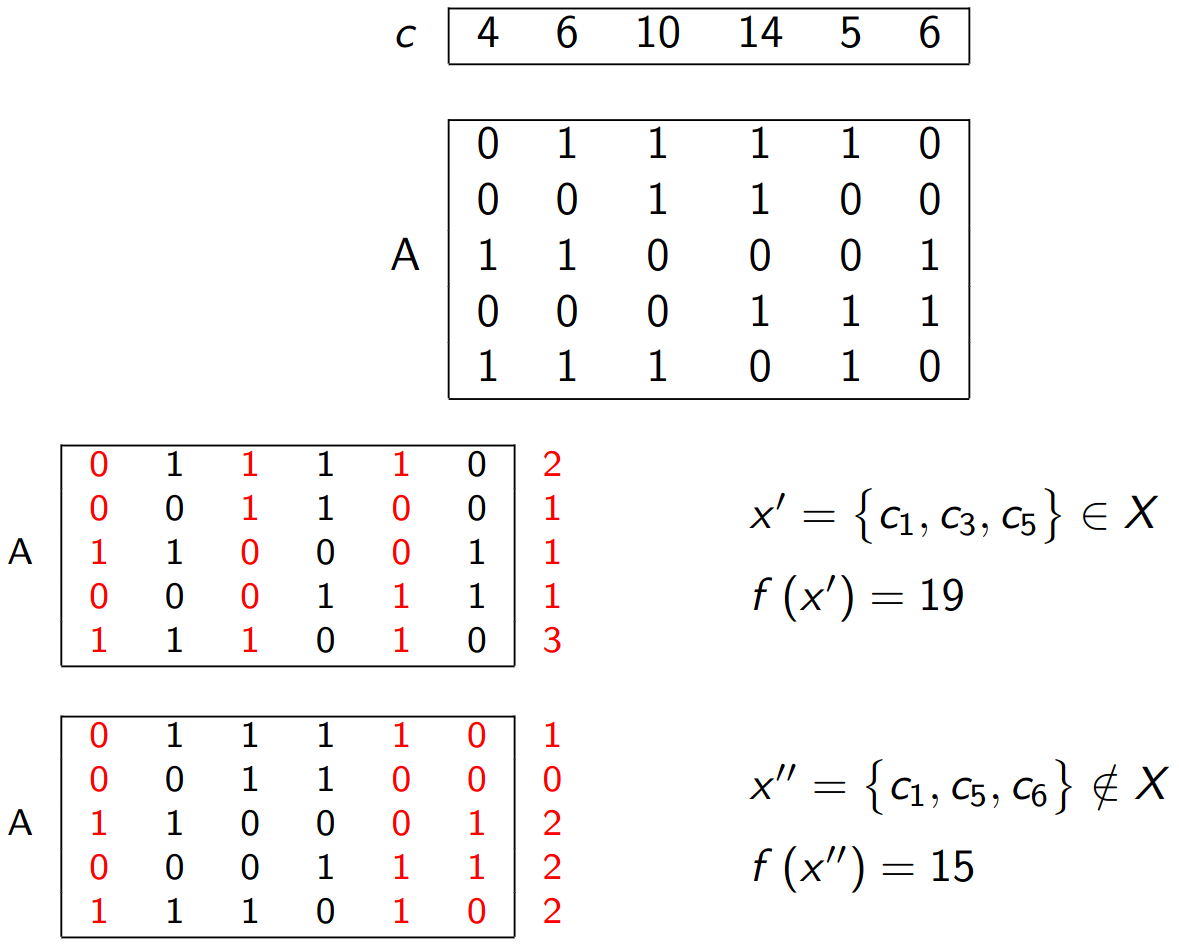
\includegraphics[width=\columnwidth]{img/SCP1}
\end{center}
The first one is a solution, the second one is unfeasible.\\

"Set Covering": covering a set (rows) with subsets (columns).\\

\newpage

\subsection*{Interlude 3: The feasibility test}
\addcontentsline{toc}{subsection}{Interlude 3: The feasibility test}
Often heuristic algorithms require solving the problem "here is a subset of elements, \textbf{is it feasible?}" or in short "$x \in X$?". It's a decision problem.\\

Sometimes is really easy (Max-SAT problem, just check that each variable appears exactly once), sometimes it's not as linear (SCP, you need the sum of each row, still easy but not \textit{as easy}).\\

The \textbf{feasibility test} requires to \textbf{compute from the solution} and test
\begin{itemize}
	\item \textbf{a single number:} the total volume (KP), the cardinality (MDP)
	\item \textbf{a single set of numbers:} values assigned to each variable (Max-SAT), number of machines for each task (PMSP)
	\item \textbf{several sets of numbers:} number of containers for each object and total volume of each container (BPP)
\end{itemize}
\nn

The time required can be \textbf{different} if the test is performed
\begin{itemize}
	\item \textbf{from scratch} on a generic subset $x$
	\item on a \textbf{subset} $x'$ obtained by slightly \textbf{modifying} a feasible solution $x$
\end{itemize}
\nn

Some modifications can be forbidden \textit{a priori} to avoid unfeasibility (insertions and removals for MDP, PMSP, Max-SAT), while others require an \textit{a posteriori} test (exchanges). Some families of modification can be ruled out.\\

% End of L1P2

\newpage

%\subsection{Numerical matrix problems}
\subsubsection{Set Packing}
Given:
\begin{itemize}
	\item a \textbf{binary matrix} $A \in \mathbb{B}^{m,n}$ with \textbf{row set} $R$ and \textbf{column set} $C$
	\item \textbf{columns} $j'$ e $j'' \in C$ \textbf{conflict} with each other when $a_{ij'} = a_{ij''} = 1$
	\item a function $\phi : \, C \rightarrow \mathbb{N}$ provides the \textbf{value of each column}
\end{itemize}
Select a \textbf{subset} of \textbf{non-conflicting columns} of \textbf{maximum value}.\\
There can't be two 1s in the same row of two chosen columns; the sum of all values in each row must be $\leq 1$.\\

The \textbf{ground set} is the set of \textbf{columns}, $B = C$.\\

The \textbf{feasible region} includes all \textbf{subsets} of \textbf{non-conflicting columns}
$$ X = \left\{x \subseteq B: \, \sum_{j \in x} a_{ij} \leq 1 \; \forall i \in R \right\}$$

The \textbf{objective} is to \textbf{maximize the total value} of the selected columns
$$ \max_{x \in X} f(x) = \sum_{j \in x} \phi_j $$

\newpage

\paragraph{Example}
\begin{center}
	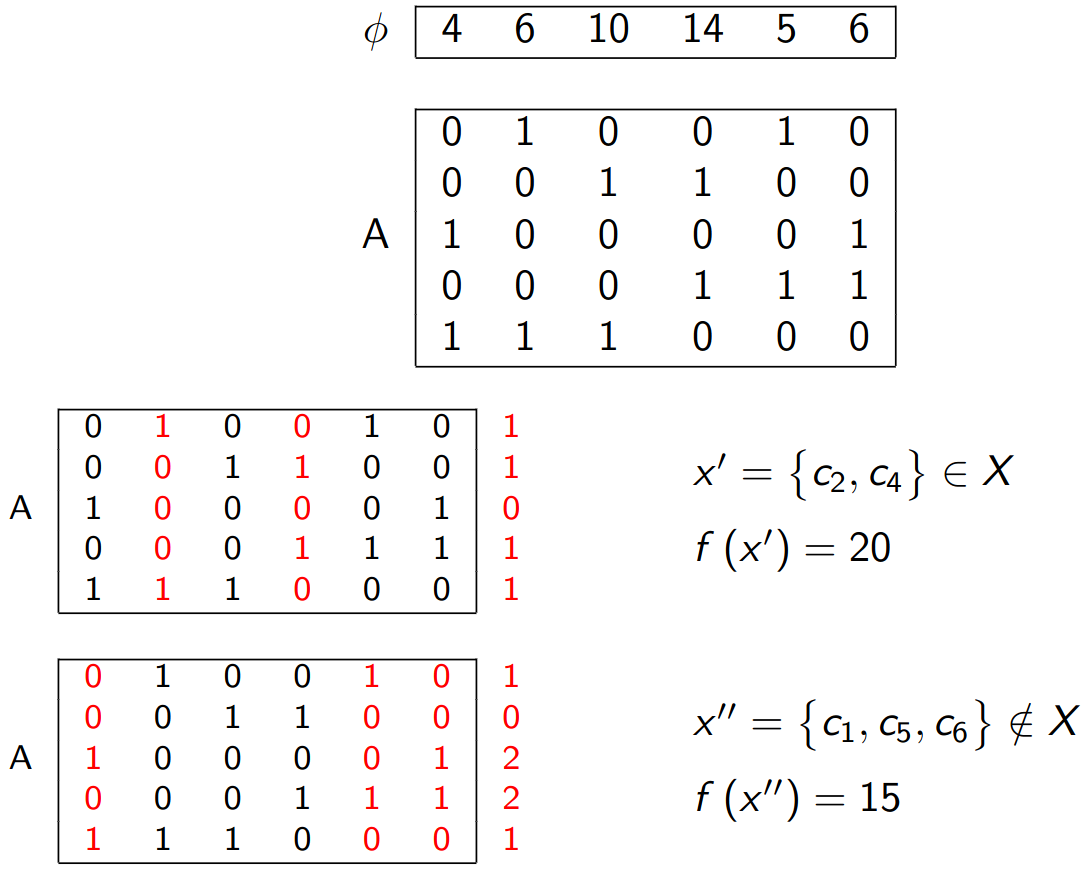
\includegraphics[width=\columnwidth]{img/SetPacking1}
\end{center}
The first one is a feasible solution, while the second one is not feasible (the sum two of the rows is $>1$).\\

"Set Packing": packing disjoint subsets (columns) of a set (rows).\\

\newpage

\subsubsection{Set Partitioning (SPP)}
Given a binary matrix and a cost function defined on its columns, select a \textbf{minimum cost} subset of \textbf{non-conflicting columns covering all rows}. It consists of:
\begin{itemize}
	\item a \textbf{binary matrix} $A \in \mathbb{B}^{m,n}$ with a \textbf{set of rows} $R$ and a \textbf{set of
		columns} $C$
	\item a function $c : \, C \rightarrow \mathbb{N}$ that provides the \textbf{cost of each column}
\end{itemize}
similar to the last problems, the difference is that the sum in each row must be exactly $= 1$; cover each row exactly once, not at least once (SCP) or at most once (Set Packing).\\

The \textbf{ground set} is the set of columns, $B = C$.\\

The \textbf{feasible region} includes all subsets of \textbf{columns} that \textbf{cover all rows} and are \textbf{not conflicting}
$$ X = \left\{x \subseteq C : \, \sum_{j \in x} a_{ij} = 1 \; \forall i \in R \right\}$$

The \textbf{objective} is to \textbf{minimize} the total \textbf{cost} of the selected \textbf{columns}
$$ \min_{x \in X} f(x) = \sum_{j \in x} c_j $$

\newpage

\paragraph{Example}
\begin{center}
	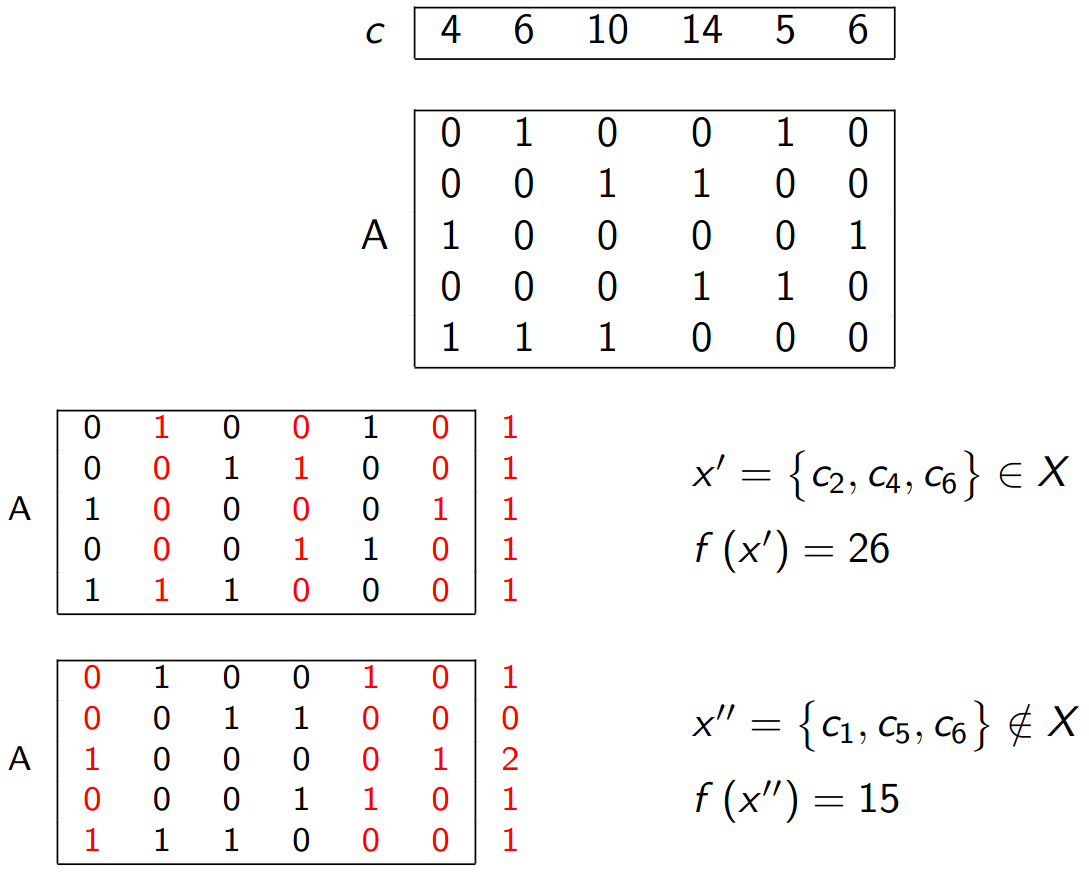
\includegraphics[width=\columnwidth]{img/SPP1}
\end{center}
The first one is a feasible solution, while the second one is not feasible (the sum of a row is $0$, while another one is $2$).\\

"Set Partitioning": partition a set (rows) into subsets (columns).\\

\newpage

\subsection*{Interlude 4: The search for feasible solutions}
\addcontentsline{toc}{subsection}{Interlude 4: The search for feasible solutions}
Heuristic algorithms often require solving the problem "\textbf{Find a feasible solution} $x \in X$", it's a search problem. \\

\textbf{Depending} on the problem, the solution can be \textbf{trivial}: 
\begin{itemize}
	\item some sets are \textbf{always feasible}, such as $x = \emptyset$ (KP, Set Packing) or $x = B$ (feasible instances of SCP)
	\item random solutions satisfying a \textbf{constraint}, such as $|x| = k$ (MDP, doesn't matter which points, you can take $k$ random points)
	\item random solutions satisfying \textbf{consistency constraints}, such as assigning one task to each machine (PMSP), one value to each logic variable (Max-SAT), etc.; a random assignment (in both cases) can be s feasible solution, it might be a bad solution, but feasible
\end{itemize}
but it can also be \textbf{hard}:
\begin{itemize}
	\item in the BPP the number of containers must be sufficiently large (e.g., provide one container for each object, then minimize)
	\item in the SPP no polynomial algorithm is known to solve the problem
\end{itemize}
Some algorithms \textbf{enlarge the feasible region} from $X$ to $X'$ (relaxation)
\begin{itemize}
	\item the \textbf{objective} $f$ must be \textbf{extended} from $X$ to $X'$ (sometimes it's possible, sometimes it's not, see first interlude)
	\item but often $X' \setminus X$ includes better solutions; the new solutions could be better (obviously, we are relaxing the constraints, the objective function can be better for unfeasible solutions)
\end{itemize}

\newpage

\subsection{Graph problems}
\subsubsection{Vertex Cover (VCP)}
Given an \textbf{undirected graph}, select a \textbf{subset of vertices of minimum cardinality} such that \textbf{each edge of the graph is incident to it}. It consists of:
\begin{itemize}
	\item an \textbf{undirected graph} $G = (V,E)$
\end{itemize}
The goal is to get every node adjacent to at least one selected node.\\
The problem can be weighted by adding a weight function to each node instead of considering unitary value.\\

The \textbf{ground set} is the \textbf{vertex set}, $B = V$.\\

The \textbf{feasible region} includes \textbf{all vertex subsets} such that \textbf{all the edges} of the graph \textbf{are incident to them}
$$ X = \left\{x \subseteq V : \, x \cap (i,j) \neq \emptyset, \;\;\; \forall (i,j) \in E \right\}$$
all the subsets of vertices such as the intersection between this and every possible pair of edges is not empty, i.e. there must be every pair of vertices in the solution.

The \textbf{objective} is to \textbf{minimize} the \textbf{number of} selected \textbf{vertices}
$$ \min_{x \in X} f(x) = |x| $$

Alternatively, the sum of the weight of the vertices, if a weight function $w$ is present
$$ \min_{x \in X} f(x) = \sum_{j \in x} w_j $$

\newpage

\paragraph{Example}
\begin{center}
	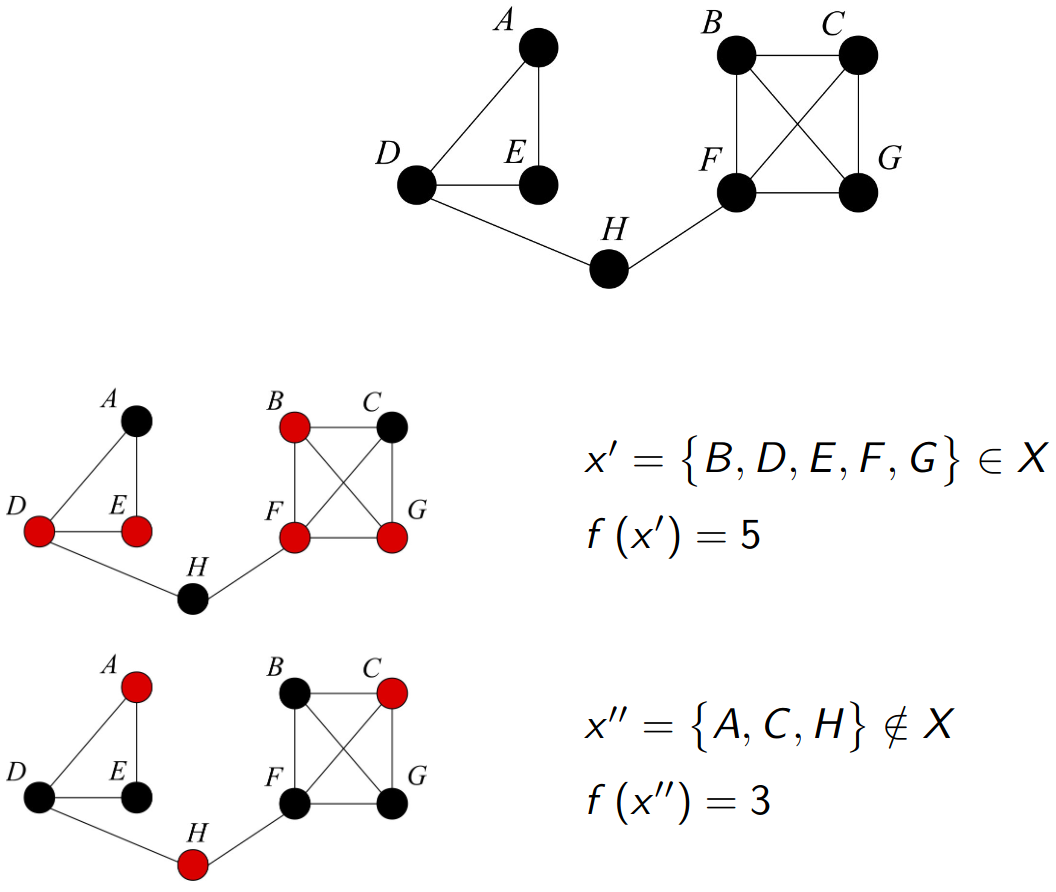
\includegraphics[width=\columnwidth]{img/VCP1}
\end{center}
The first one is a solution, the second one is unfeasible since there are some edges missing.\\
As the last interlude predicted, the unfeasible solution has a better value than the feasible one.\\

\newpage

\subsubsection{Maximum Clique Problem}
Given:
\begin{itemize}
	\item an \textbf{undirected graph} $G = (V , E )$
	\item a function $w : V \rightarrow \mathbb{N}$ that provides the weight of each vertex
\end{itemize}
select the subset of \textbf{pairwise adjacent vertices of maximum weight}.\\
The problem consists in finding the subset of adjacent vertices (a clique, each vertex is connected by an edge to every other node) of maximum weight.\\

The \textbf{ground set} is the \textbf{vertex set}, $B = V$.\\

The \textbf{feasible region} includes all \textbf{subsets of pairwise adjacent vertices}
$$ X = \left\{x \subseteq V : \, (i,j) \in E, \;\; \forall i \in x, \;\; \forall j \in X \setminus \left\{i\right\}\right\}$$
for any pair of vertices belonging to the solution the pair itself belongs to the edge set.\\

The \textbf{objective} is to \textbf{maximize} the \textbf{weight} of the selected vertices
$$ \max_{x \in X} f(x) = \sum_{j \in x} w_j $$

\newpage

\paragraph{Example}
\begin{center}
	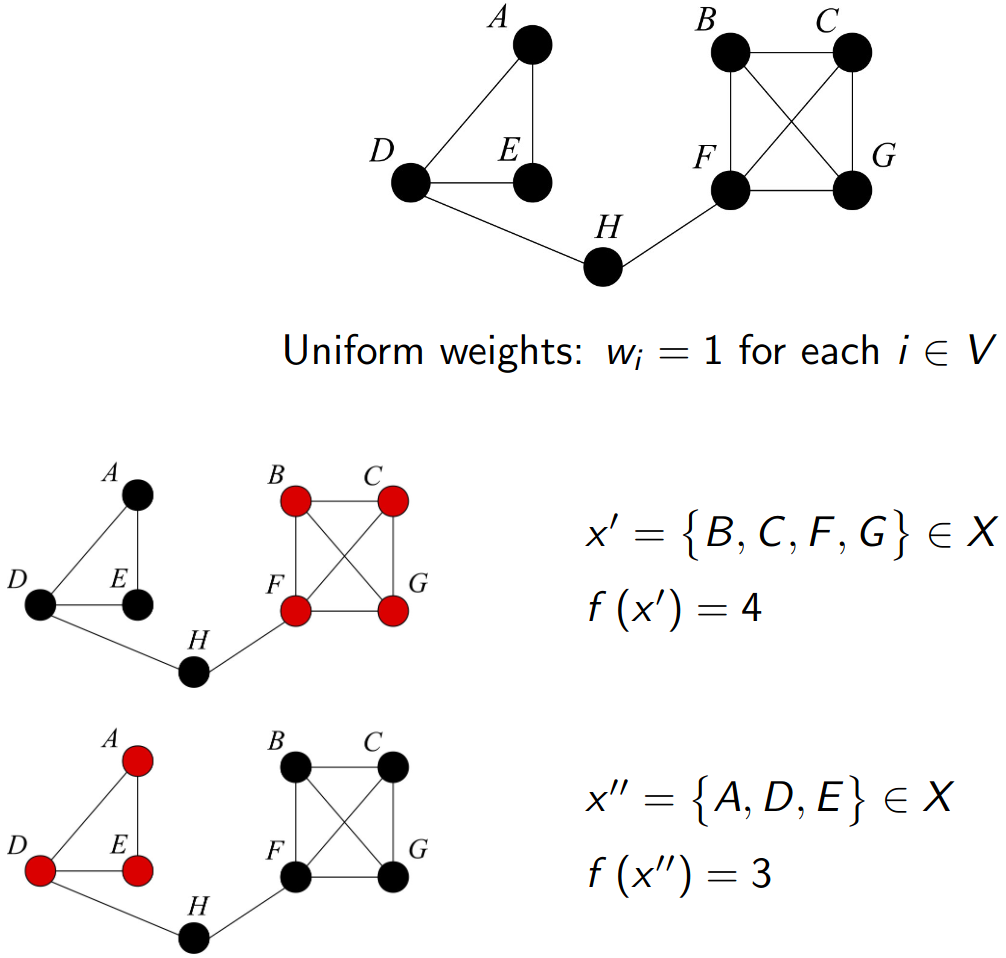
\includegraphics[width=\columnwidth]{img/MCP1}
\end{center}

\newpage

\subsubsection{Maximum Independent Set Problem}
Given
\begin{itemize}
	\item an \textbf{undirected graph} $G = (V , E )$
	\item a function $w : V \rightarrow \mathbb{N}$ that provides the \textbf{weight of each vertex}
\end{itemize}
select the \textbf{subset of pairwise nonadjacent vertices of maximum weight}.\\
The subset of not connected nodes with the maximum weight.\\

The \textbf{ground set} is the \textbf{vertex set}, $B = V$.\\

The \textbf{feasible region} includes the subsets of \textbf{pairwise nonadjacent vertices}
$$ X = \left\{x \subseteq B : \, (i,j) \notin E, \;\; \forall i \in x, \;\; \forall j \in x \setminus \left\{i\right\}\right\}$$

The \textbf{objective} is to \textbf{maximize the weight} of the selected vertices
$$ \max_{x \in X} f(x) = \sum_{j \in x} w_j $$

\newpage

\paragraph{Example}
\begin{center}
	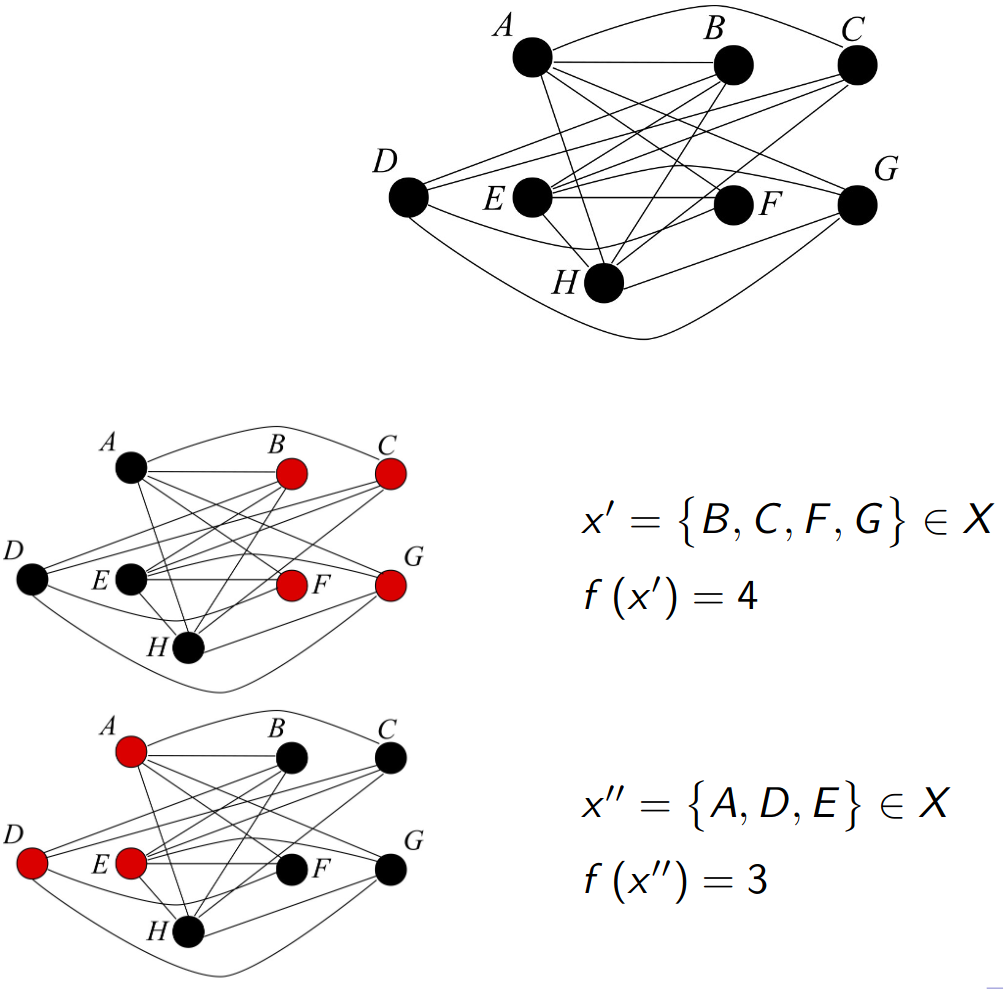
\includegraphics[width=\columnwidth]{img/MISP1}
\end{center}

\newpage

\subsection*{Interlude 5: The relations between problems}
\addcontentsline{toc}{subsection}{Interlude 5: The relations between problems}
\label{I5}
Each instance of the \textbf{MCP} is \textbf{equivalent} to an instance of the \textbf{MISP}:
\begin{enumerate}
	\item start from the MCP instance, that is graph $G = (V , E)$ \\
	\item build the complementary graph $\overline{G} = (V , (V \times V ) \setminus E )$ \\
	\item find an optimal solution of the MISP on $\overline{G}$ \\
	\item the corresponding vertices give an optimal solution of the MCP on $G$ (a heuristic MISP solution gives a heuristic MCP solution) \\
\end{enumerate}
\begin{center}
	\includegraphics[width=\columnwidth]{img/interlude5}
\end{center}
The process can also be applied in the \textbf{opposite} direction.\\

The \textbf{solution of the MCP can be used to find the solution of the MISP}, and vice versa.\\
There's no need to design two different algorithms since the same one works for both problems, with a simple transformation of the instance.\\

\newpage

The \textbf{VCP} and the \textbf{SCP} are also \textbf{related}, but in a different way; each instance of the VCP can be \textbf{transformed} into an \textbf{instance} of the SCP:
\begin{itemize}
	\item each edge $i$ corresponds to a row of the covering matrix $A$
	\item each vertex $j$ corresponds to a column of $A$
	\item if edge $i$ touches vertex $j$, set $a_{ij} = 1$; otherwise $a_{ij} = 0$
	\item an optimal solution of the SCP gives an optimal solution of the VCP (a heuristic SCP solution gives a heuristic VCP solution)
\end{itemize}
\begin{center}
	\includegraphics[width=\columnwidth]{img/interlude52}
\end{center}
The reverse is not as simple, not every binary matrix can be turned into a graph.\\

The VCP is equivalent to solving the SCP on a matrix that determines to which vertices every edge is connected to.\\

\newpage

The \textbf{BPP} and the \textbf{PMSP} are \textbf{equivalent}, but in a more sophisticated way:
\begin{itemize}
	\item the \textbf{tasks} correspond to the \textbf{objects}
	\item the \textbf{machines} correspond to the \textbf{containers}, but
	\begin{itemize}
		\item BPP: minimize the number of containers, given the capacity
		\item PMSP: given the number of machines, minimize the completion time
	\end{itemize}
\end{itemize}
Start from a \textbf{BPP instance}
\begin{enumerate}
	\item make an \textbf{assumption} on the optimal \textbf{number} of \textbf{containers} (e.g., 3)
	\item build the \textbf{corresponding PMSP} instance
	\item \textbf{compute} the \textbf{optimal} completion \textbf{time} (e.g., 95)
	\begin{itemize}
		\item if it \textbf{exceeds} the capacity (e.g., 80), increase the assumption (4 or 5)
		\item if it \textbf{does not}, decrease the assumption (2 or 1)
	\end{itemize}
	(using heuristic PMSP solutions leads to a heuristic BPP solution)
\end{enumerate}

\begin{center}
	\includegraphics[width=0.8\columnwidth]{img/interlude53}
\end{center}

The reverse process is \textit{possible}.\\

The two problems are equivalent, but each one must be solved several times.\\

\newpage

\subsubsection{Traveling Salesman Problem (TSP)}
Given:
\begin{itemize}
	\item a \textbf{directed graph} $G = (N, A)$
	\item a function $c : \, A \rightarrow \mathbb{N}$ that provides the \textbf{cost of each arc}
\end{itemize}
select a \textbf{circuit} visiting \textbf{all the nodes} of the graph at \textbf{minimum cost}.\\

The \textbf{ground set} is the \textbf{arc set}, $B = A$.\\

The \textbf{feasible region} includes the \textbf{circuits} that \textbf{visit all nodes} in the graph (Hamiltonian circuits).\\

How to determine whether a subset is a feasible solution? \\
And a modification of a feasible solution? \\
Can some modifications be ruled out? \\
Finding a Hamiltonian circuit is usually $\np$-hard, it's trivial only in the case of a connected graph. \\

The \textbf{objective} is to \textbf{minimize} the \textbf{total cost} of the selected arcs
$$ \min_{x \in X} f(x) = \sum_{j \in x} c_j $$

\newpage

\paragraph{Example}
\begin{center}
	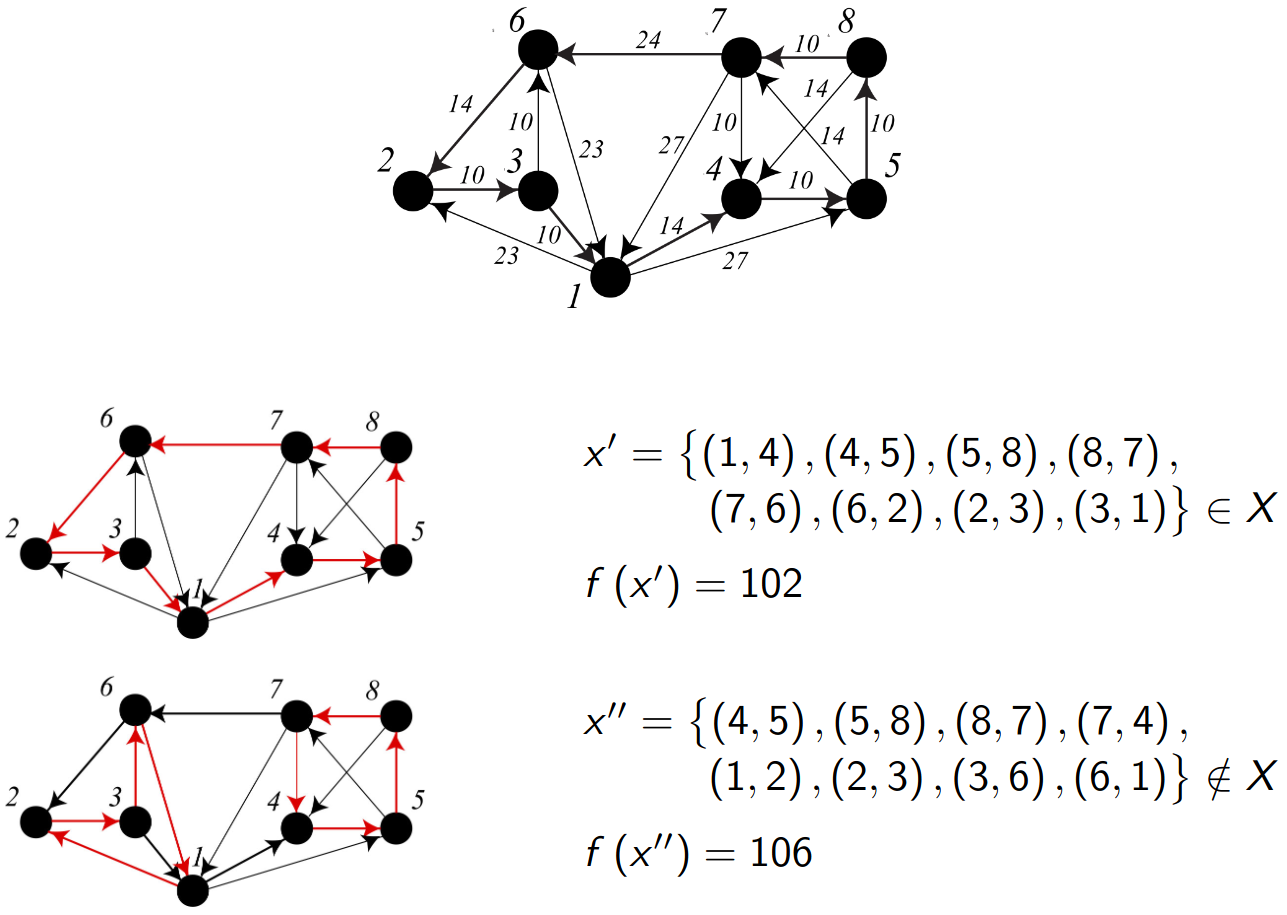
\includegraphics[width=\columnwidth]{img/TSP1}
\end{center}
The first one is a solution, the second one isn't because although it visits all the vertices there are 2 different sub-circuits.\\

\newpage

\subsubsection{Capacitated Min. Spanning Tree Problem}
Given
\begin{itemize}
	\item an \textbf{undirected graph} $G = (V , E )$ with a \textbf{root vertex} $r \in V$
	\item a function $c : \, E \rightarrow \mathbb{N}$ that provides the \textbf{cost of each edge}
	\item a function $w : \, V \rightarrow \mathbb{N}$ that provides the \textbf{weight of each vertex}
	\item a number $W \in \mathbb{N}$ that is the \textbf{subtree appended to the root} (branch), i.e., capacity of each subtree
\end{itemize}
select a \textbf{spanning tree} of \textbf{minimum cost} such that each \textbf{branch respects the capacity}.\\
Find a spanning tree starting from a root node $r$, each branch must be under the limit weight (not too many vertices, must be under $W$).\\

The \textbf{ground set} is the \textbf{edge set}, $B = E$.\\

The \textbf{feasible region} includes \textbf{all spanning trees} such that the \textbf{weight of the vertices} spanned by each branch \textbf{does not exceed} $W$.\\
The feasibility test requires to visit the subgraph.\\

The \textbf{objective} is to \textbf{minimize} the \textbf{total cost} of the selected edges
$$ \min_{x \in X} f(x) = \sum_{j \in x} c_j $$

\newpage

\paragraph{Example}
\begin{center}
	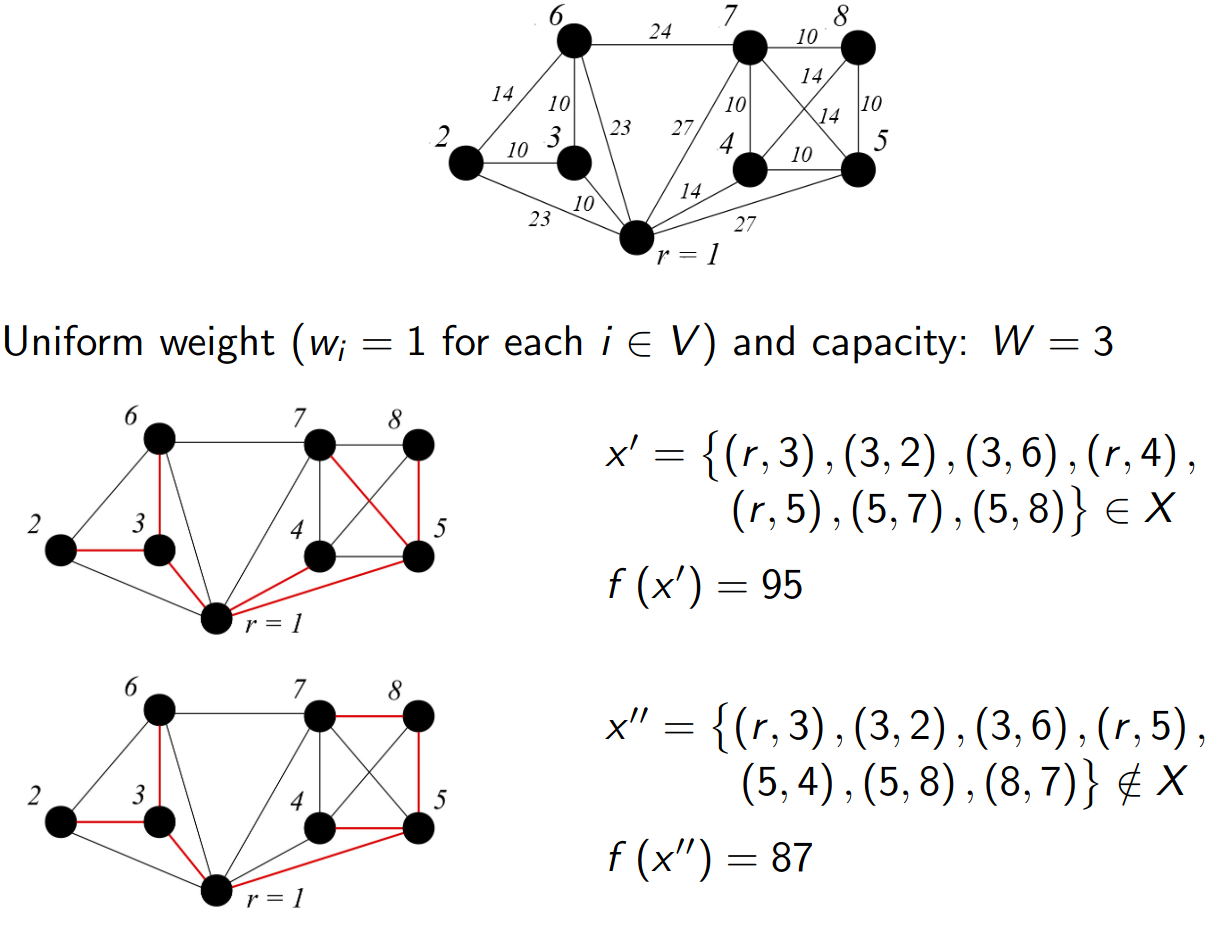
\includegraphics[width=0.8\columnwidth]{img/CSTP}
\end{center}
It is easy to evaluate the objective, less easy the feasibility.

\paragraph{Cost of the main operation:} the objective function is:
\begin{itemize}
	\item \textbf{fast to evaluate:} sum the edge cost
	\item \textbf{fast to update:} sum the added costs and subtract the removed ones
\end{itemize}
but it's easy to generate nonoptimal subtrees given the covered vertices.\\

The \textbf{feasibility test} is
\begin{itemize}
	\item \textbf{not} very \textbf{fast to perform:} 
	\begin{itemize}
		\item visit to check for connection and acyclicity
		\item visit to compute the total weight of each subtree
	\end{itemize}
	\item \textbf{not} very \textbf{fast to update:} 
	\begin{itemize}
		\item show that the removed edges break the loops introduced by the added ones
		\item recompute the weights of the subtrees
	\end{itemize}
\end{itemize}
This also holds when the graph is complete.\\

What if we described the problem in terms of vertex subsets?

\newpage

\paragraph{Alternative description:} Define a set of \textbf{subtrees} $T$ (as in the containers in the BPP), one for each vertex in $V \setminus \left\{r\right\}$: some can be empty.\\

The \textbf{ground set} is the \textbf{set of the (vertex,branch) pairs}, $B = V \times T$.\\

The \textbf{feasible region} includes \textbf{all partitions of the vertices into connected subsets} (visit, trivial on complete graphs) \textbf{of weight} $\leq W$ (as in the BPP)
$$ X = \left\{x \subseteq B : \, |x \cap B_v| = 1, \;\; \forall v \in V \setminus \left\{r\right\}, \, \sum_{(i,j)\in B^t} w_i \leq W \; \forall t \in T, \; ... \; \right\}$$
with $B_v = {(i, j) \in B : \, i = v }$, $B^t = {(i, j) \in B : j = t}$.\\

The \textbf{objective} is to \textbf{minimize} the \textbf{sum of the costs of the branches} spanning each subset of vertices and appending it to the root.\\
It is a combination of minimum spanning tree problems.\\

The previously considered solutions now have a \textbf{different representation}.
\begin{center}
	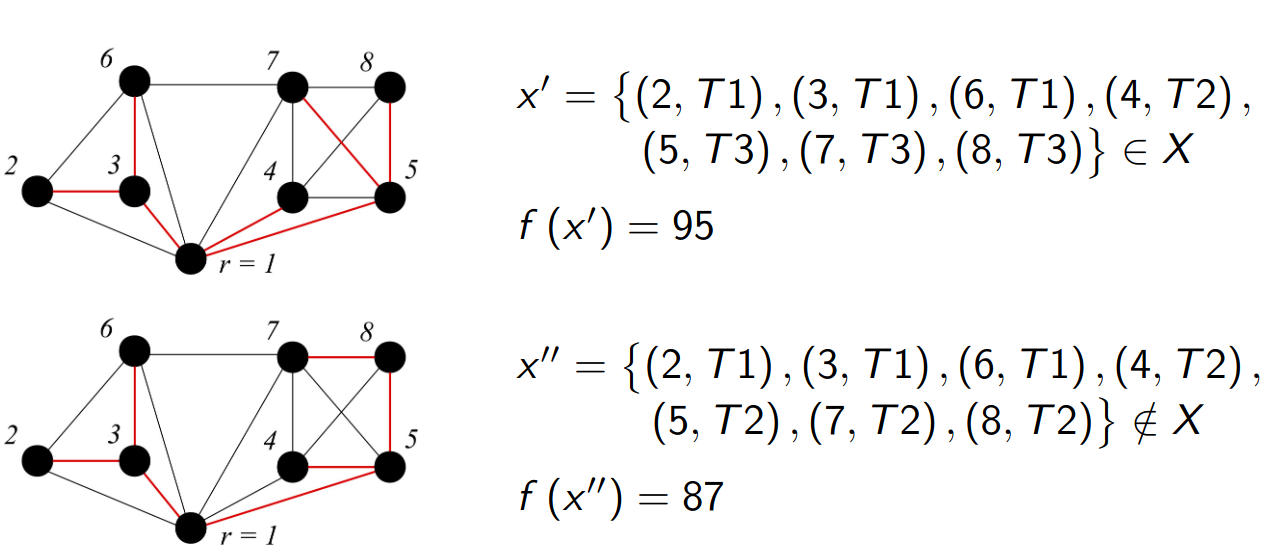
\includegraphics[width=0.9\columnwidth]{img/CSTP2}
\end{center}
The feasibility test only requires summing the weights, computing the objective requires solving a MST problem.

\newpage

\paragraph{New cost of operations:} The objective function is
\begin{itemize}
	\item \textbf{slow to evaluate:} compute a MST for each subset
	\item \textbf{slow to update:} recompute the MST for each modified subset
\end{itemize}
but the subtrees are \textbf{optimal by construction}.\\

If the graph is complete, the \textbf{feasibility test} is
\begin{itemize}
	\item \textbf{fast to perform:}
	\begin{itemize}
		\item sum the weights of the vertices for each subtree
	\end{itemize}
	\item \textbf{fast to update:}
	\begin{itemize}
		\item sum the added weights and subtract the removed ones
	\end{itemize}
\end{itemize}
There are advantages and disadvantages switched places.\\

\newpage

\subsubsection{Vehicle Routing Problem (VRP)}
Given
\begin{itemize}
	\item a \textbf{directed graph} $G = (N, A)$ with a \textbf{depot node} $d \in N$
	\item a function $c : A \rightarrow \mathbb{N}$ that provides the \textbf{cost of each arc}
	\item a function $w : N \rightarrow \mathbb{N}$ that provides the \textbf{weight of each node}
	\item a number $W \in \mathbb{N}$ that is the \textbf{capacity of each circuit}
\end{itemize}
select a \textbf{set of circuits} of \textbf{minimum cost} such that \textbf{each one visits the depot and respects the capacity}.\\
It's a set of circuits visiting all the nodes, if the TSP had more salesmen and each salesman has a maximum capacity of stuff he can bring.\\

The \textbf{ground set} could be
\begin{itemize}
	\item the \textbf{arc set}, $B = A$
	\item the \textbf{set of all (node,circuit) pairs}, $B = N \times C$
\end{itemize}

The \textbf{feasible region} could include
\begin{itemize}
	\item all \textbf{arc subsets} that \textbf{cover all nodes} with circuits \textbf{visiting the depot} and whose \textbf{weight does not exceed} $W $(again the visit of a graph)
	\item all \textbf{partitions} of the nodes into \textbf{subsets of weight non larger than} $W$ and \textbf{admitting a spanning circuit} (NP-hard problem)
\end{itemize}

The \textbf{objective} is to \textbf{minimize the total cost} of the selected arcs
$$ \min_{x \in X} f(x) = \sum_{j \in x} c_j $$

\newpage

\paragraph{Example}
\begin{center}
	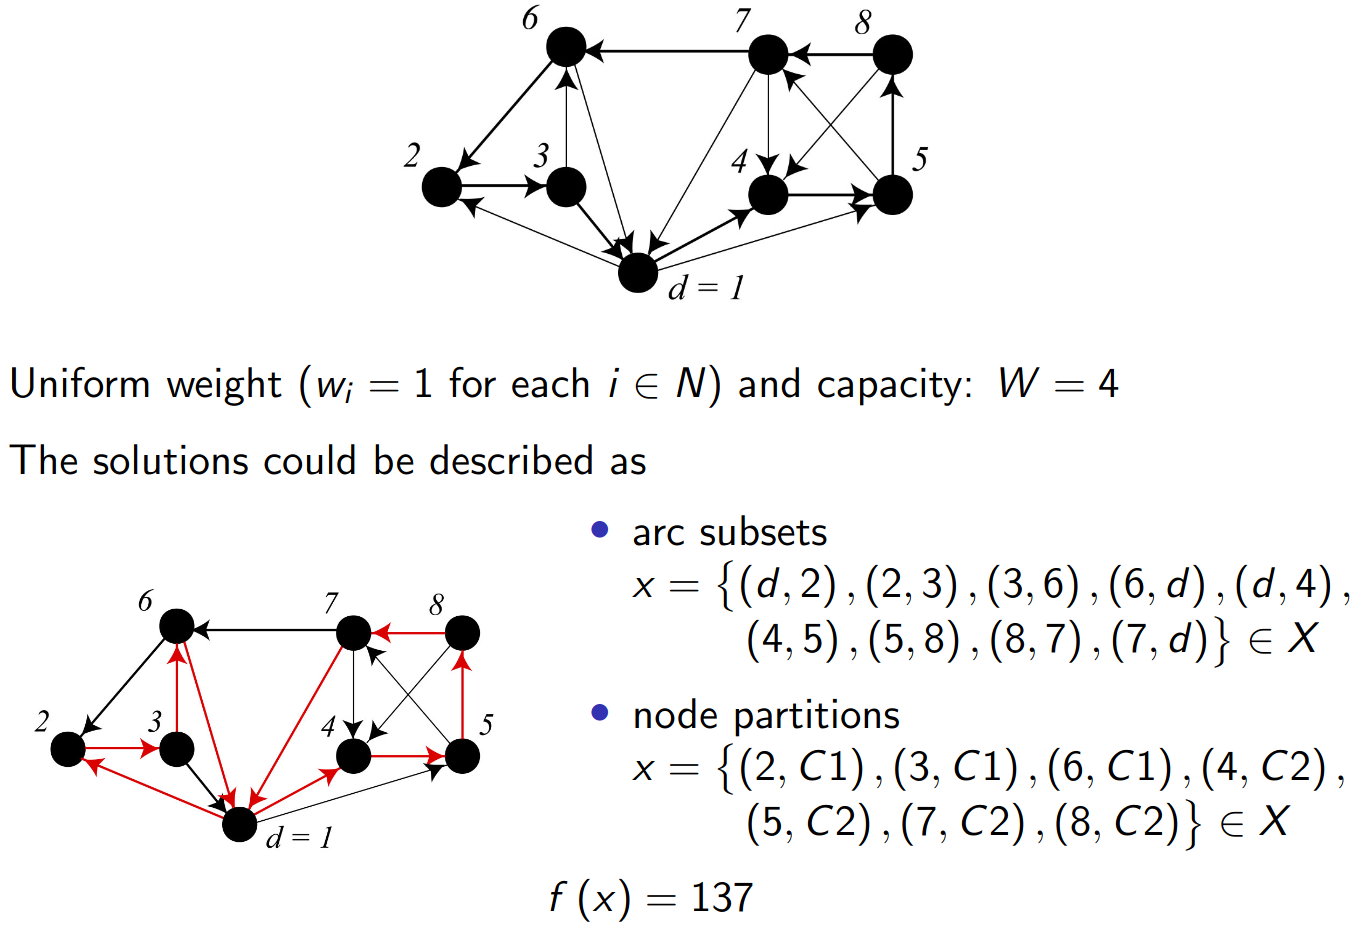
\includegraphics[width=0.9\columnwidth]{img/VRP1}
\end{center}

\newpage

\subsection*{Interlude 6: Combining alternative representations}
\addcontentsline{toc}{subsection}{Interlude 6: Combining alternative representations}
The \textbf{CMSTP} and the \textbf{VRP} share an interesting complication: \textbf{different definitions of the ground set} $B$ are possible and natural
\begin{itemize}
	\item the description as a \textbf{set of edges/arcs} looks preferable to \textbf{manage the objective}
	\item the description as a \textbf{set of pairs (vertex,tree)/(node,circuit)} looks better to \textbf{generate optimal solutions and to deal with feasibility}
\end{itemize}

Which description should be adopted?
\begin{itemize}
	\item the one that makes easier the most frequent operations
	\item both, if they are used much more frequently than updated, so that the burden of keeping them up-to-date and consistent is acceptable
\end{itemize}

% End of L2

\newpage